%!TEX TS-program = ../make.zsh

\section{Discussion}
\label{sec:discussion}

\subsection{Comparison to Other Hole-Ice-Simulation Methods}
\label{sec:comparison_methods}

\subsubsection{A Priori Modification of Angular-Acceptance Curves}
\label{sec:a_priori_modification_of_angular_acception_curves}\label{sec:a_priori_curve}

% https://github.com/fiedl/hole-ice-study/issues/10

Using a modified angular-acceptance curve $a(\eta)$ as acceptance criterion of the optical modules in simulations to effectively account for the effect of hole ice on the detection of photons, is the default approach in \clsim (see sections \ref{sec:a_priori_angular_acceptance} and \ref{sec:hole_ice_approximation}).

\docpar{Information on the nominal and the hole-ice-approximating angular-acceptance curves are provided or linked in \issue{10}.}

The respective angular-acceptance curves have been obtained using lab measurements and simulations using the \photonics photon-propagation software. \cite{icepaper, lundberg, photonics}

Figure \ref{fig:Wee4ahYa} shows three modified angular-acceptance curves that approximate the hole-ice effect in comparison to the optical module's angular acceptance based on the lab measurement. The modified curves H1, H2, and H3 assume that the entire drill hole is filled with hole ice, corresponding to a hole-ice-cylinder radius of $30\cm$, and assume geometric hole-ice scattering lengths of $\lambda\sca\hi = 100\cm$ (H1), $\lambda\sca\hi = 50\cm$ (H2), and $\lambda\sca\hi = 30\cm$ (H3) respectively.

\begin{figure}[htbp]
  % https://github.com/fiedl/hole-ice-study/issues/113
  \smallerimage{angular-acceptance-h0-h1-h2-h3}
  \caption{A priori angular-acceptance curves: \underline{blue}: without hole ice, \underline{H1}: assuming a hole-ice-cylinder radius if $30\cm$ and a geometric hole-ice scattering length of $\lambda\sca\hi = 1.00\m$, corresponding to an effective hole-ice scattering length of $\lambda\esca\hi = 16.67\m$, \underline{H2}: $\lambda\sca\hi = 0.50\m, \lambda\esca\hi = 8.33\m$, \underline{H3}: $\lambda\sca\hi = 0.30\m, \lambda\esca\hi = 5.00\m$. \cite{icepaper, yag, icemodelsdata}}
  \label{fig:Wee4ahYa}
\end{figure}

Using modified angular-acceptance curves for the optical modules to approximate the hole-ice effect has the advantage that new parameters gained from calibration studies can be inserted into the existing simulations just by replacing the polynomial parameters used for the angular acceptance of the optical modules.

Also, using modified acceptance curves is faster than simulating the hole ice directly as the many scattering steps that correspond to the photons scattering within the hole ice are not actually simulated and just effectively accounted for using when the algorithm decides whether a photon hit is accepted by an optical module.

This method, however, relies on strong assumptions: The lab measurements the acceptance curves are based on, have been performed using manufactured ice rather than South-Polar ice. The hole-ice modifications are based purely on simulations and do not use any \icecube calibration information. \cite{icepaper}

Furthermore, this method assumes all optical modules having exactly the same properties regarding positioning and relative orientation. The optical modules are assumed to be perfectly centered within the drill hole as well as in the bubble column.

The a priori H2 acceptance curve, which is used in standard-\clsim simulations by default, is used as reference curve for other angular-acceptance plots in this study.

However, comparing this reference curve, which itself assumes a hole-ice-cylinder radius of $30\cm$ and a geometric scattering length of $50\cm$ (H2 parameters) \cite{icemodelsdata}, to a \clsim simulation using the same H2 parameters (figure \ref{fig:iQu2aBuz}), both angular-acceptance curves do not match. Instead, the reference curve best matches a \clsim simulation, which assumes a hole-ice radius of the same size as the optical module, $r = 0.1651\m$, and an effective hole-ice scattering length of $\lambda\esca\hi \approx 1.0\m$ (section \ref{sec:parameter_scan}).

\begin{figure}[htbp]
  \subcaptionbox{\clsim simulation with H2 hole-ice parameters:\\ $r = 30\cm, \lambda\sca\hi = 50\cm, \lambda\sca\hi = 8.33\m$}{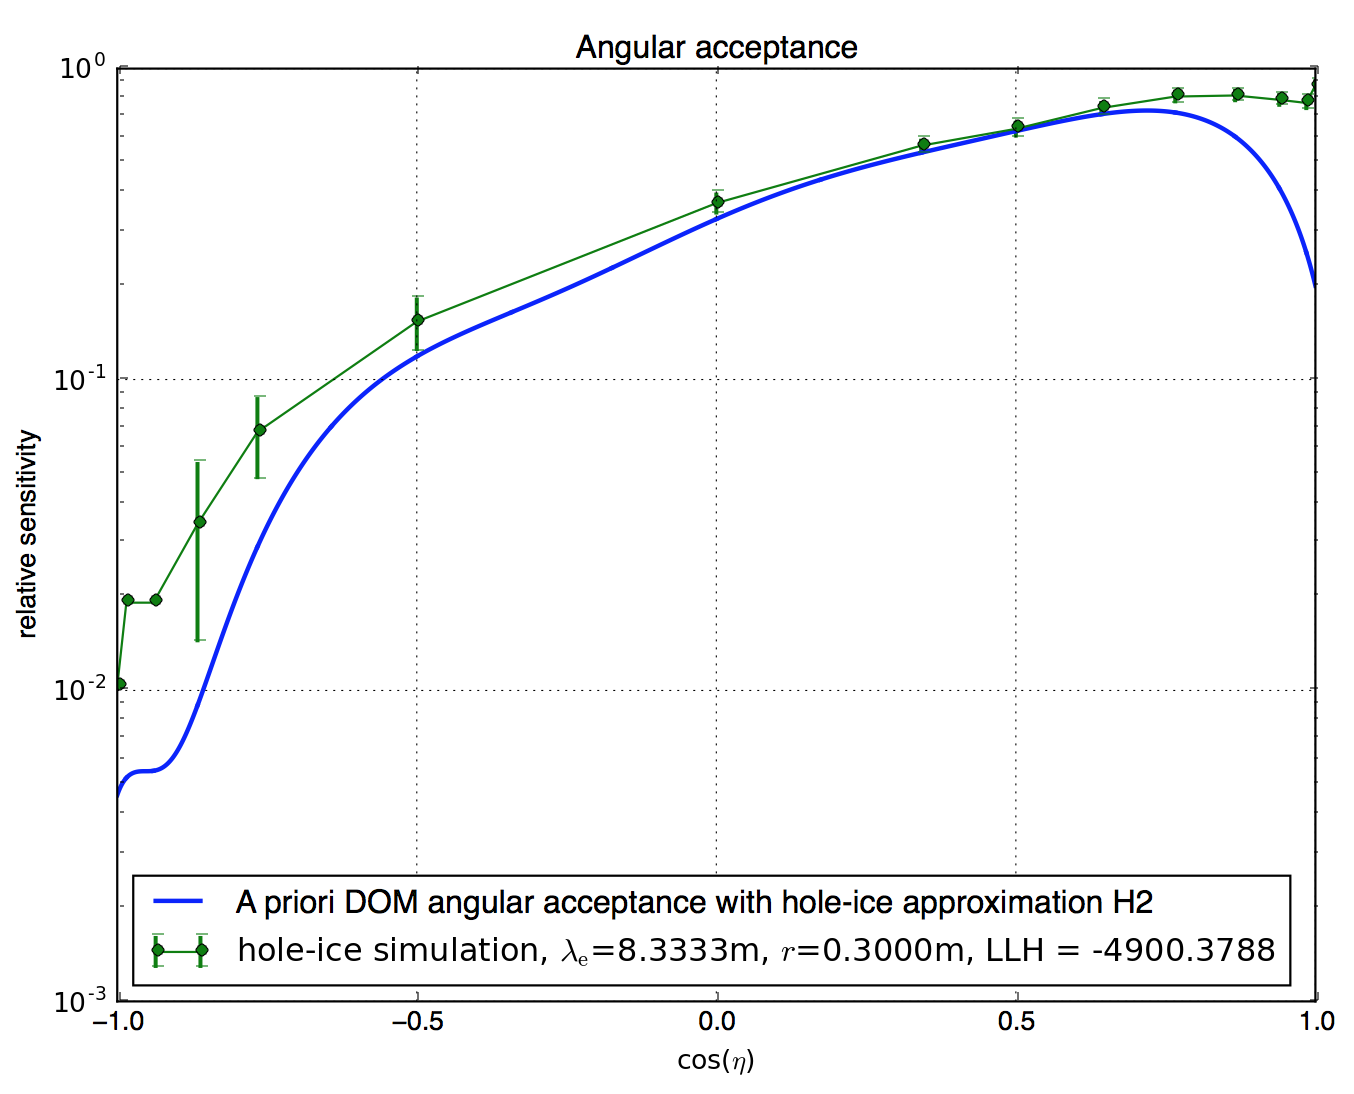
\includegraphics[height=0.27\textheight]{img/angular-acceptance-karle-h2-vs-reference-alt}}\hfill
  \subcaptionbox{\clsim simulation with parameters\\ $r = r\dom = 0.1651\m, \lambda\sca\hi = 6\cm, \lambda\esca\hi = 1.0\m$}{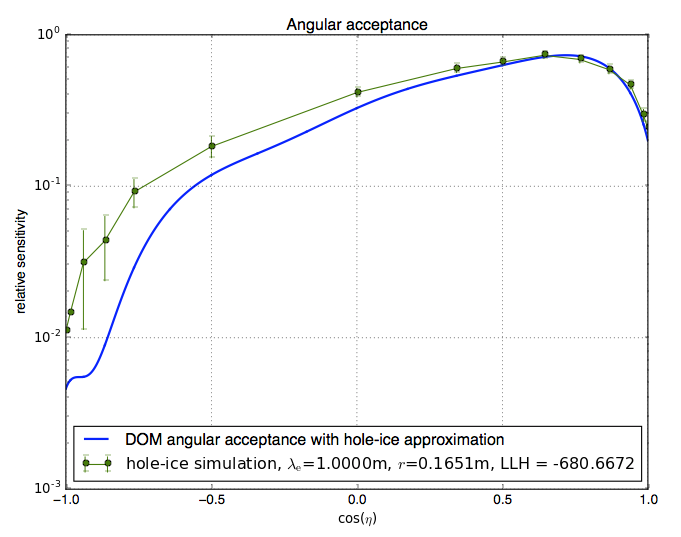
\includegraphics[height=0.27\textheight]{img/parameter-scan-1-1-angular}}\hfill
  \caption{Comparing the a priori angular-acceptance curve assuming H2 hole-ice parameters from \cite{icepaper,yag} to \clsim simulations.}
  \label{fig:iQu2aBuz}
\end{figure}


\subsubsection{Angular-Acceptance Fitting Using Flasher Data}
\label{sec:dimas_model}

% Dima's model
% https://github.com/fiedl/hole-ice-study/issues/102
%
% Flasher unfolding, flasher fits
% \cite{flasherdataderivedicemodels}
%
% d.h. man nimmt nicht Eis-Eigenschaften an, sondern fittet die Winkelakzeptanz direkt an Flasher-Daten
%
% https://wiki.icecube.wisc.edu/index.php/MSU_Forward_Hole_Ice
%
% Another advantage of using Dima's hole ice instead of H2 to extend the parametrization is that
% Dima's hole ice has a somewhat simple formula with a single parameter p as systematic, while the
% H2 model was made via fitting the angular acceptance curve of different simulated hole ices with
% different scattering lengths which means each of the fits turned out somewhat different as seen in
% the figure above and one parametrization would not be as easily transferable to the hole ice at
% different scattering parameters.
%
\chirkin suggests a hole-ice model, often referred to as \textit{Dima's model}, resulting in an angular-acceptance curve, $a\domdima(\eta;p)$, different from the a priori curves for the H1, H2, H3 models. \cite{flasherdataderivedicemodels}

\question{Is \enquote{Dima's model} ok: Is this colloquial or a terminus technicus?}

The curve is parameterized using a single parameter $p\in\reals$ that has been determined as $p \in [0.2;0.4]$ using flasher studies. \cite{msuforwardholeice} In this model, the properties $\HH$ of the hole ice, that is to say the hole-ice-cylinder radius $r$ and the scattering length $\lambda\sca\hi$ within the hole ice are unknown.\footnote{As the hole-ice parameters are not given by Dima's model, one cannot directly compare the model to \clsim simulations with direct hole-ice propagation. A parameter scan to find the best hole-ice parameters for Dima's model is suggested as follow-up study. See: \url{https://github.com/fiedl/hole-ice-study/issues/114} \followup}

\begin{align}
  a\domdima(\eta;p) = & \ 0.34 \cdot (1 + 1.5\,\cos(\eta) - \cos(\eta)^{\sfrac{3}{2}}) \nonumber \\
      & + p \cdot \cos(\eta) \cdot  (\cos(\eta)^2 - 1)^3 \\
      & \ p \in [0.2;0.4] \nonumber
  \label{eq:adima}
\end{align}

Figure \ref{fig:Vohn9Oov} shows this angular-acceptance curve, $a\domdima(\eta;p)$, for the parameters $p=0.2$, $p=0.3$, and $p=0.4$, compared to the a priori angular-acceptance curve $a\domhi(\eta)$ of the H2 model and the angular-acceptance curve of an optical module $a\dom(\eta)$ without hole ice.

\begin{figure}[htbp]
  \smallerimage{h2-vs-dima-vs-h0-102}
  \caption{Comparing the a priori angular-acceptance curve H2 from \cite{icepaper} to Dimas's model \cite{flasherdataderivedicemodels}. Also, the angular acceptance of the optical module (DOM) without any hole ice is shown.}
  \label{fig:Vohn9Oov}
\end{figure}

Notably, the effect of the hole ice on photons approaching the optical module directly from above or below is weaker in this model compared to the H2 approximation curve. However, the overall acceptance in the lower half sphere is higher, and the overall acceptance in the upper half sphere is lower as in the H2 approximation curve.

This approach does not rely on specific assumptions about the properties of the hole ice, but uses flasher calibration data to measure the mean angular-acceptance behavior of \icecube's optical modules.

Nevertheless, this method relies on the same assumptions regarding the equality of all optical modules: All optical modules are assumed to have the same relative position and orientation with respect to the hole ice.


\subsubsection{Direct Photon Propagation With \ppc}
\label{sec:direct_photon_propagation_with_ppc}\label{sec:pocam}

\chirkin and \rongen have performed simulations with direct propagation through hole ice, similar to this study, but using \ppc for the photon propagation rather than \clsim. \cite{martinspicehddard, martindardupdate, pocam, icrc17pocam, ppcpaper}

\sourcepar{The source code of \ppc can be found at \url{http://code.icecube.wisc.edu/projects/icecube/browser/IceCube/projects/ppc}.}

Simulating the propagation of photons through the hole ice by simulating the scattering directly drops the assumption that all optical modules need to be equally positioned and oriented with respect to the hole ice. All optical modules can be individually calibrated using flasher data. \cite{martinspicehddard}

The basic propagation algorithm is the same in \ppc and \clsim. The algorithm for propagating the photons through different media, relies on the same principle of converting randomized numbers of interaction lengths to a geometric distances, but is implemented differently: Ice layers and hole-ice cylinders are hard-coded in \ppc whereas in \clsim's new medium-propagation algorithm, they are treated as generic medium changes (see section \ref{sec:algorithm_b}). Both, \ppc and \clsim, can be run on clusters of graphics processing units. \cite{ppcpaper, ppcsource, ppcforhumans, clsimsource}

Hardware requirements and performance of \ppc and \clsim are comparable. Due to micro optimizations, \ppc tends to run slightly faster.\footnote{Internal correspondence suggests a performance factor of 1.5 to 2.0. See also section \ref{sec:performance} for performance considerations.}

\ppc does only support one hole-ice cylinder per string. The main cable of the detector string is not implemented as absorbing object but rather accounted for by using a direction-dependent shadowing factor for incoming photons. \cite{ppcsource, ppcforhumans}
In particular, the cable cannot be modeled to reside inside the bubble-column cylinder. \cite{martinspicehddard}
% martinspicehddard, slide 39:
% > Current cable implementation deletes photon from
% > a given range of azimuthal impact directions
% > → cable is not allowed to be inside bubble
% > → check with Sweden camera deployment footage
% > Implement cable as asecond independent cylinder

Since both propagation softwares, \ppc and \clsim with the new medium-propagation mechanism, are performing the same task, it is important to know whether both simulations produce the same or similar results regarding the effect of the hole ice. A detailed comparison of \ppc and \clsim results is out of scope of this study. But a first comparison can be achieved using existing \ppc simulation results.\followup

In feasibility studies for the proposed \noun{Precision Optical CAlibration Module} (\noun{POCAM}), direct photon propagation simulations with \ppc have been performed, assuming different hole-ice parameters, and producing effective angular-acceptance curves corresponding to those hole-ice parameters. \cite{pocam, icrc17pocam}

Assuming the same hole-ice parameters respectively, angular-acceptance simulations can be performed in \clsim, allowing for a direct comparison of the \ppc and the \clsim results (figure \ref{fig:Ou7fux1o}).

\docpar{The \clsim angular-acceptance simulations with hole-ice parameters from the \noun{POCAM} simulations are documented in \issue{103}.}

\begin{figure}[htbp]
  \subcaptionbox{No hole ice in both simulations.}{\halfimage{pocam-no-hole-ice}}\hfill
  \subcaptionbox{Hole-ice-cylinder radius $r = 0.6\,r\dom = 10\cm$, hole-ice effective scattering length $\lambda\esca\hi = 14\cm$, corresponding to a geometric scattering length $\lambda\sca\hi = 0.8\cm$ in both simulations.}{\halfimage{pocam-06rdom-esca14cm}}\hfill
  \subcaptionbox{Hole-ice-cylinder radius $r = 1.8\,r\dom = 30\cm$, hole-ice effective scattering length $\lambda\esca\hi = 125\cm$, corresponding to a geometric scattering length $\lambda\sca\hi = 7.5\cm$ in both simulations.}{\halfimage{pocam-18rdom-esca125cm}}\hfill
  \subcaptionbox{Hole-ice-cylinder radius $r = 1.8\,r\dom = 30\cm$, hole-ice effective scattering length $\lambda\esca\hi = 170\cm$, corresponding to a geometric scattering length $\lambda\sca\hi = 10.2\cm$ in both simulations.}{\halfimage{pocam-18rdom-esca170cm}}\hfill
  \caption{Comparison of effective angular-acceptance curves, which include hole-ice effects for varying hole-ice parameters, created with two independent propagation tools, \ppc and \clsim. As reference, the a priori effective angular-acceptance curve for H2 parameters from \cite{icepaper} is shown. Data source of the \ppc simulations is a series of \noun{POCAM} simulations \cite{icrc17pocam}. The radius of the optical module is $r\dom = 16.510\cm$. Both simulations roughly agree, but the \clsim simulation sees more photons for angles with $\cos \eta < 0.5$.}
  \label{fig:Ou7fux1o}
\end{figure}

At a rough view, both simulations produce similar effective angular-acceptance results for different hole-ice parameters. For upper angles, however, this study's simulation systematically sees more photon hits than \ppc. As this has already been observed in section \ref{sec:angular_acceptance_simulations_without_hole_ice} (see figure \ref{fig:Shai8yah}) when introducing plane waves as photon sources, this effect could be a systematic problem of the implementation of the angular-acceptance simulations rather than of the propagation algorithm.

Further investigations on this matter are required, but are out of scope of this study.\followup


\subsection{Comparison to Hole-Ice Parameters From Other Studies}
\label{sec:angular_acceptance_comparison}\label{sec:parameter_comparison}

% https://github.com/fiedl/hole-ice-study/issues/104

\newcommand\ok{\ding{51}} %\checkmark
\newcommand\same{\cellcolor{black!25}}
\newcommand\greyedout{\cellcolor{black!25}}
\newcommand\bad{\ding{55}}

\newcommand\clsimppc{\noun{clsim+ppc}}

Simulations with direct photon propagation through hole ice of different parameter configurations $\HH$ allow to rate the compatibility of different hole-ice models. For example, generating simulation-based angular-acceptance curves allows to calculate the likelihood of two models being compatible. This, however, would require a more involved study of systematics of the specific simulation design, which is out of scope of this study, but should be considered by follow-up studies.\followup

As a first step, however, angular-acceptance curves from simulations with hole-ice parameters from different studies are shown in this section. Table \ref{tab:angular_acceptance_compatibility} at the end of this section (page \pageref{tab:angular_acceptance_compatibility}) summarizes the findings.


% https://github.com/fiedl/hole-ice-study/issues/80
%
% Albrecht Karle, Hole Ice Studies with YAG, 1998:
% http://icecube.berkeley.edu/kurt/interstring/hole-ice/yak.html
%
% This YAG laser analysis suggests that the hole ice is described
% best by a geometric scattering length in the range between 50 cm and 100 cm
%
% Hole ice models
% Model 0: hole ice identical to bulk ice
% Model 1: L_scatt = 100 cm (missing in this analysis)
% Model 2: L_scatt = 50 cm
% Model 3: L_scatt = 30 cm
% Model 4: L_scatt = 10 cm
% Scattering length = geometric scattering length on air bubbles.
% Hole diameter = 60 cm.
%
% https://wiki.icecube.wisc.edu/index.php/Hole_ice
%
% These were derived many years ago, and are characterised by the scattering length of the bubble
% column. The H2 model is typically referred to as the "baseline" model, which corresponds to a
% scattering length of 50cm. In simulation, the effects of the H* models are parametrised via angular
% acceptance curves (see above) that determine the probability to accept a photon based on its arrival
% direction (not position) when it intersects with the DOM surface. The derivation of these angular
% acceptance curves assumed that the entire drill hole is full of the scattering centres. However from
% the Sweden camera images we suspect that this hypothesis is incorrect, and the bubbles instead
% concentrate in the centre of the drill hole rather than throughout.
%
\subsubsection{YAG H2 Parameters}
\label{sec:yag_h2_parameters}
Based on laser measurements, using a Yttrium-Aluminium-Granat (YAG) laser, \authorname{Karle} suggested a number of hole-ice models \cite{holeicestudieswithyag}, from which the so called \textit{H2 model} has become the dominant hole-ice model in \icecube. This model suggests a geometric scattering length of $50\cm$ for the hole ice, and a hole-ice-cylinder radius of $30\cm$, and is the basis for the modified angular-acceptance curve with hole-ice approximation described in section \ref{sec:a_priori_modification_of_angular_acception_curves}.

Using the new direct photon propagation though hole ice with \clsim, one can simulate the propagation through hole ice with parameters suggested by the H2 model, scan the angular acceptance of an optical module within the simulation, and compare the result to the existing a priori angular-acceptance curve (section \ref{sec:a_priori_curve}) as well as the angular-acceptance curve suggested by Dima's model (section \ref{sec:dimas_model}).

\docpar{This angular-acceptance simulation using the H2 hole-ice parameters is documented in \issue{80}.}

Figure \ref{fig:xaeg2Mee} shows the result of this angular-acceptance simulation in comparison to the a priori angular-acceptance curve with hole-ice approximation \cite{icepaper} and Dima's model \cite{flasherdataderivedicemodels}.

\begin{figure}[htbp]
  \smallerimage{angular-acceptance-karle-h2-xaeg2Mee}
  \caption{Angular-acceptance simulation with hole-ice parameters from the so called \textit{H2 model} \cite{holeicestudieswithyag}, which describes the hole ice as cylinder of $30\cm$ radius filling the entire drill hole, with a geometric scattering length of $50\cm$, corresponding to an effective scattering length of $\lambda\hi\esca = 8.33\m$, using the new medium-propagation algorithm (section \ref{sec:algorithm_b}) with direct detection as acceptance criterion and plane waves as photon sources. In comparison, the a priori angular-acceptance curve from \cite{icepaper} and the angular-acceptance curve of Dima's model \cite{flasherdataderivedicemodels} are shown.}
  \label{fig:xaeg2Mee}
\end{figure}

For photons approaching the optical module from below (right-hand side of the plot), the simulation rather follows Dima's model, but counts more detected photons in total. For photons approaching from above (left-hand side of the plot), the form of the simulation curve is similar to the a priori curve, in particular with respect to the plateau on the left hand side, but, again, the simulation counts more photons in total.


\subsubsection{\noun{DARD} Parameters}
\label{sec:dard_parameters}

In the \noun{DARD} study (\noun{Data Acquisition for a flasheR DOM}), LED measurements are used to determine the hole-ice properties. The different flasher LEDs of an optical module are turned on in sequence, and the light detected by the same DOM is measured. The process is then compared to detailed \noun{Geant4} simulations for different hole-ice parameters in order to find the optimal hole-ice parameters to explain the data. \cite{martindardupdate, martinspicehddard}

The \noun{DARD} study assumes a fixed hole-ice radius of $r=30\cm$. The best fit value for the geometric scattering length of the hole ice has been determined as $\lambda\hi\sca = 10\cm$, which is considerably lower than other estimates. \cite{martindardupdate}

Using the new direct photon propagation though hole ice with \clsim, one can simulate the propagation through hole ice with parameters suggested by \noun{DARD}, scan the angular acceptance of an optical module within the simulation, and compare the result to the existing a priori angular-acceptance curve as well as the angular-acceptance curve suggested by Dima's model.

\docpar{This angular-acceptance simulation for the hole-ice parameters suggested by the \noun{DARD} study, is documented in \issue{105}.}

Figure \ref{fig:eePai1sh} shows the result of this angular-acceptance simulation in comparison to the a priori angular-acceptance curve with hole-ice approximation \cite{icepaper} and Dima's model \cite{flasherdataderivedicemodels}.

\begin{figure}[htbp]
  \smallerimage{angular-acceptance-dard-eePai1sh}
  \caption{Angular-acceptance simulation with hole-ice parameters from the \noun{DARD} study \cite{martindardupdate}, which suggest a hole-ice cylinder of $30\cm$ radius and a geometric scattering length of $\lambda\sca\hi = 10\cm$, corresponding to an effective scattering length of $\lambda\hi\esca = 1.67\m$, using the new medium-propagation algorithm (section \ref{sec:algorithm_b}) with direct detection as acceptance criterion and plane waves as photon sources. In comparison, the a priori angular-acceptance curve from \cite{icepaper} and the angular-acceptance curve of Dima's model \cite{flasherdataderivedicemodels} are shown.}
  \label{fig:eePai1sh}
\end{figure}

For photons approaching the optical module from below (right-hand side of the plot), the simulation curve rather follows the a priori acceptance curve, but shows a less sharp hole-ice drop-off effect. For $\cos\eta < 0.5$, that is to say for higher angles, the simulation registers relatively more photons, both in comparison to the a priori curve and to Dima's model.


\subsubsection{\noun{SpiceHD} Parameters}
\label{sec:spicehd_parameters}

The \noun{SpiceHD} study (\noun{South Pole ICE model with Hole ice fitting and Direct detection}) uses flasher data and direct photon propagation simulations with \ppc to determine the parameters of the hole ice. In this 7-string flasher study, LED flashes are sent from a central optical module and the numbers and time distributions of photon hits are observed at the optical modules of the six surrounding strings.\footnote{\noun{SpiceHD} uses the same methods as \cite{icepaper,dimaslikelihood}}
% correspondance 2018-08-17
% https://icecube-spno.slack.com/archives/D092M93E3/p1534500882000100

Comparing the flasher data to simulations with different hole-ice parameters, that is to say scanning over the hole-ice-cylinder radius and the hole-ice scattering length, a range of hole-ice parameters is found to be suitable (section \ref{sec:spicehd_flasher_scan_contours}). When assuming a compatible hole-ice column radius as observed by camera images \cite{rongenswedishcamera}, the best fit hole-ice parameters have been determined as a hole-ice-cylinder radius of $60\,\%$ of the radius of an optical module, $r = 0.6\,r\dom = 10\cm$, and the hole-ice effective scattering length $\lambda\esca\hi = 14\cm$, which corresponds to a geometric scattering length of $\lambda\sca\hi = 0.84\cm$, which is even smaller than the geometric scattering length of $10\cm$ suggested by \noun{DARD}. \cite{martinspicehddard}

Using the new direct photon propagation though hole ice with \clsim, one can simulate the propagation through hole ice with parameters suggested by \noun{SpiceHD}, scan the effective angular acceptance of an optical module within the simulation, and compare the result to the existing a priori angular-acceptance curve \cite{icepaper} as well as the angular-acceptance curve suggested by Dima's model \cite{flasherdataderivedicemodels} (figure \ref{fig:ku3Zie8z}).

\docpar{This angular-acceptance simulation for the hole-ice parameters suggested by the \noun{SpiceHD} study, is documented in \issue{87}.}

\begin{figure}[htbp]
  \smallerimage{angular-acceptance-splicehd-ku3Zie8z}
  \caption{Angular-acceptance simulation with hole-ice parameters suggested by the \noun{SpiceHD} study \cite{martinspicehddard}: The dominant hole ice is assumed as a bubble column with radius $r = 0.6\,r\dom$ where $r\dom$ is the radius of the optical module. The bubble column is thinner than the optical module. The hole-ice effective scattering length is $\lambda\esca\hi = 14\cm$. The simulation uses the new medium-propagation algorithm (section \ref{sec:algorithm_b}) with direct detection as acceptance criterion and plane waves as photon sources. The simulation results are shown in comparison with the a priori angular-acceptance curve from \cite{icepaper} and the angular-acceptance curve of Dima's model \cite{flasherdataderivedicemodels}.}
  \label{fig:ku3Zie8z}
\end{figure}

For photons that approach the optical module from below (right-hand side of the plot in figure \ref{fig:ku3Zie8z}), the simulation shows a hole-ice effect between the a priori curve and Dima's model. For photons approaching from above, the simulation shows a plateau. For $\cos\eta < 0.5$, the simulation shows more photon hits than both, the a priori curve and Dima's model.


\subsubsection{\noun{SpiceHD} Flasher-Scan Contours}
\label{sec:spicehd_flasher_scan_contours}

The \noun{SpiceHD} study (\noun{South Pole ICE model with Hole ice fitting and Direct detection}, see also section \ref{sec:spicehd_parameters}) performs a similar flasher study as described in section \ref{sec:flasher}.

Both studies compare simulations using direct photon propagation through hole ice of varying parameters to flasher calibration data. This study uses the new medium-propagation algorithm for \clsim, \noun{SpiceHD} uses \ppc to propagate the photons. The parameter-scan results for both studies are shown in figure \ref{fig:ahCoHee4}.

\begin{figure}[htbp]
  \subcaptionbox{\noun{SpiceHD} study using direct hole-ice propagation with \ppc \cite{martinspicehddard}}{\halfimage{flasher-contours-martin}}\hfill
  \subcaptionbox{Flasher study with direct hole-ice propagation with \clsim (section \ref{sec:flasher})}{\halfimage{flasher-contours-59-alt}}
  \caption{Fitting flasher simulations for different hole-ice parameters to calibration data. Both studies show a similar qualitative behavior. Due to a number of systematics (section \ref{sec:flasher}), the fitted parameters of (b) are not to be trusted.}
  \label{fig:ahCoHee4}
\end{figure}

Both studies show a ``valley''-like region of good agreement of data and simulation. Above the valley, that is to say for longer scattering lengths or smaller hole-ice radii, the simulated hole ice is too weak. Below the valley, the simulated hole ice is too strong. However, both, the parameter region of the valley and the curvature are different.

As \clsim and \ppc show good agreement when comparing angular-acceptance curves (section \ref{sec:pocam}), this difference is most probably due to systematics of the preliminary flasher study, discussed in section \ref{sec:flasher}. Most notably, the optical module is centered within the hole ice in the \clsim flasher simulation, whereas \noun{SpiceHD} has fitted the position of the optical module relative to the hole ice. Estimations show that this difference can account for a factor of $3$ for the scattering length.

% from 7-string LED flasher studies \cite{martinspicehddard} and camera observations \cite{rongenswedishcamera}, $r = 0.6\,r\dom = 10\cm$, $\lambda\sca = 0.84\cm$, $\lambda\esca = 14\cm$ (section \ref{sec:spicehd_parameters}

This leaves the hole-ice parameters from the \noun{SpiceHD} study \cite{martinspicehddard} that best match the camera observations \cite{rongenswedishcamera}, $r = 0.6\,r\dom = 10\cm$, $\lambda\sca = 0.84\cm$, $\lambda\esca = 14\cm$ (section \ref{sec:spicehd_parameters}), as the favorable hole-ice parameters for now.
\subsubsection{Compatibility of Hole-Ice Models}
\label{sec:compatibility_of_hole_ice_parameters}

Direct photon-propagation-simulation through hole ice allows to compare different hole-ice models and hole-ice parameters.
Both photon-propagation-simulation tools, \ppc and \clsim, produce matching effective angular-acceptance curves for direct photon propagation through hole ice. For photons approaching the optical module from above, the systematic uncertainties of the \clsim angular-acceptance scans appear too large to consider this angular range. Therefore, this section focuses on the angular range $\cos \eta > 0$ with large statistics, when assessing the compatibility of different hole-ice models.

The \noun{SpiceHD} flasher study is compatible to camera observations. The resulting hole-ice parameters $\HH_\text{SpiceHD}$ as well as the parameters $\HH_\text{YAG H2}$ suggested by earlier laser calibration studies, both suggest a weaker hole-ice effect than approximated in the modified a priori angular-acceptance curve used in standard \clsim simulations. Dima's hole-ice model that only uses flasher-calibration data and does not rely on direct hole-ice simulations, also suggests a weaker hole ice. Using the hole-ice parameters $\HH_\text{DARD}$ in direct hole-ice simulations, suggested by the single-LED calibration study \noun{DARD}, however, results in angular-acceptance curves similar to the a priori angular-acceptance curve. Table \ref{tab:angular_acceptance_compatibility} shows a summary (page \pageref{tab:angular_acceptance_compatibility}).

This leaves no obvious conclusion on which current hole-ice model is to be preferred. But as both direct hole-ice-simulation tools produce compatible results, both tools can now be used to study the various hole-ice scenarios in detail.

\begin{table}[p]
  \begin{center}
  \resizebox{\columnwidth}{!}{%
  \begin{tabular}{rr|ccccccc}
                            & \small{\textbf{Method}}     & \clsimppc           & \clsimppc         & \clsimppc            & A priori   & Dima \\
    \small{\textbf{Method}} & \small{\textbf{Parameters}} & $\HH_\text{YAG H2}$ & $\HH_\text{DARD}$ & $\HH_\text{SpiceHD}$ & $\HH_\text{YAG H2}$ & -- \\
    %                        & $r$                         & \\
    %                        & $\lambda\sca\hi$            & \\
    %                        & $\lambda\esca\hi$           & \\
    \hline
    \clsimppc               & $\HH_\text{YAG H2}$         & \same               & \greyedout        & \greyedout           & \greyedout & \greyedout \\
    \clsimppc               & $\HH_\text{DARD}$           & \bad                & \same             & \greyedout           & \greyedout & \greyedout \\
    \clsimppc               & $\HH_\text{SpiceHD}$        & \ok                 & \bad              & \same                & \greyedout & \greyedout \\
    A priori                & $\HH_\text{YAG H2}$         & \bad                & \ok               & \bad                 & \same      & \greyedout\\
    Dima's model            & --                          & \ok                 & \bad              & \ok                  & \bad       & \same
  \end{tabular}
  }
  \end{center}
  \caption{Compatibility of angular-acceptance curves $a(\eta)$. \textbf{Methods}: \underline{\clsim}: Angular-acceptance simulation with \clsim using the new medium-propagation algorithm with plane waves as photon sources and direct detection as acceptance criterion (section \ref{sec:angular_acceptance_scan}). \underline{\ppc}: POCAM-angular-acceptance simulation with \ppc using direct photon propagation through hole ice and direct detection (section \ref{sec:direct_photon_propagation_with_ppc}). \underline{\clsimppc}: Simulations performed with both, \clsim and \ppc, producing similar results. \underline{A priori}: A priori angular-acceptance curve $a\domhi(\eta)$ for $\HH_\text{YAG H2}$ parameters from \cite{icepaper} (section \ref{sec:hole_ice_approximation}). \underline{Dima}, \underline{Dima's model}: Angular-acceptance curve $a\domdima(\eta;p)$ from flasher unfolding studies \cite{flasherdataderivedicemodels} (section \ref{sec:dimas_model}). \textbf{Hole-Ice Parameters}: Each parameter set $\HH$ consists of a hole-ice-cylinder radius $r$ and a geometric hole-ice scattering length $\lambda\sca$, corresponding to an effective scattering length $\lambda\esca$. \underline{$\HH_\text{YAG H2}$}: from YAG laser measurements \cite{holeicestudieswithyag}, also called H2 model parameters, $r = 30\cm, \lambda\sca=50\cm, \lambda\esca = 8.33\m$ (section \ref{sec:yag_h2_parameters}). \underline{$\HH_\text{DARD}$}: from single-DOM LED measurements \cite{martindardupdate}, $r=30\cm$, $\lambda\sca = 10\cm, \lambda\esca = 1.67\m$ (section \ref{sec:dard_parameters}). \underline{$\HH_\text{SpiceHD}$}: from 7-string LED flasher studies \cite{martinspicehddard} and camera observations \cite{rongenswedishcamera}, $r = 0.6\,r\dom = 10\cm$, $\lambda\sca = 0.84\cm$, $\lambda\esca = 14\cm$ (section \ref{sec:spicehd_parameters}). \textbf{Rating}: \ok: Curves look roughly similar. \bad: Curves do not look similar.}
  \label{tab:angular_acceptance_compatibility}
\end{table}